\documentclass{article}
\usepackage{amssymb}
\usepackage{graphicx}
\usepackage{hyperref}
\usepackage[left=1.5cm, right=1.5cm]{geometry}

\hypersetup{
    colorlinks=true,
    linkcolor=blue,
    filecolor=magenta,      
    urlcolor=cyan,
}

\makeatletter
\renewcommand\subsection{\@startsection{subsection}{2}{\z@}%
                                     {-3.25ex\@plus-1ex \@minus-.2ex}%
                                     {1.5ex \@plus.2ex}%
                                     {\normalfont\normalsize\bfseries}}
\makeatother

\renewcommand{\contentsname}{Indice} % Change the title of the table of contents

% chktex-file 44
\title{QuickHospital}
\author{}
\date{}

\renewcommand{\labelenumi}{\arabic{enumi}.}
\renewcommand{\labelenumii}{\arabic{enumi}.\arabic{enumii}.}
\renewcommand{\labelenumiii}{\arabic{enumi}.\arabic{enumii}.\arabic{enumiii}.}
\renewcommand{\labelenumiv}{\arabic{enumi}.\arabic{enumii}.\arabic{enumiii}.\arabic{enumiv}.}
\begin{document}

\maketitle

\tableofcontents

\newpage

\section{Specifica}

\begin{enumerate}
    \item persona
    \begin{enumerate}
        \item nome
        \item cognome
        \item data nascita
    \end{enumerate}
    \item medico
    \begin{enumerate}
        \item pazienti che hanno in cura
        \item specializzazione primaria
        \item specializzazioni secondarie
    \end{enumerate}
    \item paziente
    \begin{enumerate}
        \item recapiti telefonici
        \item email (unica)
        \item recapito postale (unico)
    \end{enumerate}
    \item stanza
    \begin{enumerate}
        \item i posti letto (da 1 a 8)
        \item piano int $>$ 0
        \item settore int $>$ 0
    \end{enumerate} 
    \item posto letto
    \item ricovero
    \begin{enumerate}
        \item paziente
        \item posto letto
        \item dataora
    \end{enumerate}
    \item dimissione
    \begin{enumerate}
        \item dataora dimissione
    \end{enumerate}
    \item specializzazione
    \begin{enumerate}
        \item nome
    \end{enumerate}
    \item prestazione
    \begin{enumerate}
        \item data richiesta
        \item descrizione
        \item medico che la eroga
        \item specializzazione richiesta
    \end{enumerate}
\end{enumerate}

\newpage
\section{Analisi}
\subsection{Diagramma delle classi}
\begin{figure}[h]
    \centering
    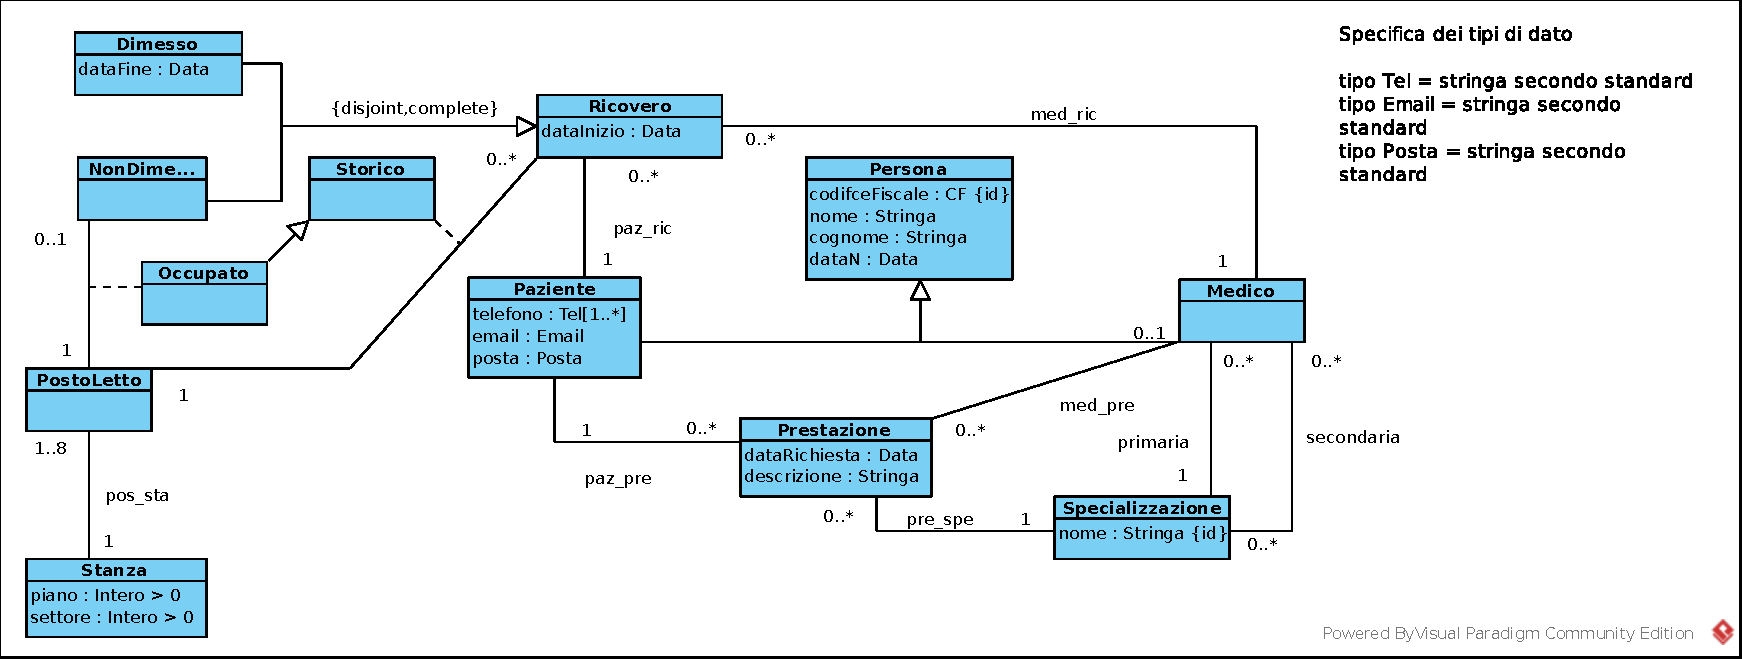
\includegraphics[width=1\textwidth]{./Diagrammi/analisi.pdf}
    \caption{Analisi}
\end{figure}

\newpage

\subsection{Dizionario dei dati}

\begin{itemize}
    \item tel = stringa secondo standard
    \item cf = stringa alfanumerica secondo standard
    \item email = stringa secondo standard
    \item posta = stringa secondo standard
\end{itemize}

\newpage

\subsection{Vincoli}

\begin{itemize}
    \item \textbf{[V.Prestazione.medico\_giusto]}\\
    Ogni medico associato a una prestazione ha la specializzazione richiesta dalla prestazione:
    \[
    \forall m,p,s \; (med\_pre(m,p) \land pre\_spe(p,s) \rightarrow (primaria(m,s) \lor secondaria(m,s)))
    \]
    
    \item \textbf{[V.Medico.secondaria\_non\_primaria]}\\
    Se un medico è associato a una specializzazione secondaria, non può essere associato alla stessa specializzazione come primaria:
    \[
    \forall s,m \; (secondaria(m,s) \rightarrow \neg primaria(m,s))
    \]
    
    \item \textbf{[V.Dimesso.date\_consistente]}\\
    Se un paziente è dimesso, la data di inizio del ricovero deve essere precedente o uguale alla data di fine:
    \[
    \forall r \; (Dimesso(r) \rightarrow \forall d_1,d_2 \; (dataInizio(r,d_1) \land dataFine(r,d_2) \rightarrow d_1 \leq d_2))
    \]
    
    \item \textbf{[V.Ricovero.date\_consistente]}\\
    La data di inizio del ricovero deve essere successiva o uguale alla data di nascita del paziente:
    \[
    \forall r,dr,p,dp \; (paz\_ric(p,r) \land dataInizio(r,dr) \land dataN(p,dp) \rightarrow dr \geq dp)
    \]
    
    \item \textbf{[V.Prestazione.date\_consistente]}\\
    La data di richiesta della prestazione deve essere successiva o uguale alla data di nascita del paziente:
    \[
    \forall paz,pre,d1,d2 \; (paz\_pre(paz,pre) \land dataRichiesta(pre,d1) \land dataN(paz,d2) \rightarrow d1 \geq d2)
    \]
    
    \item \textbf{[V.Medico.date\_consistente]}\\
    La data di inizio del ricovero deve essere successiva alla data di nascita del medico:
    \[
    \forall m,r,d1,d2 \; (med\_ric(m,r) \land dataInizio(r,d1) \land dataN(m,d2) \rightarrow d1 > d2)
    \]
    
    \item \textbf{[V.Paziente.ricovero\_singolo]}\\
    Un paziente può avere un solo ricovero non dimesso alla volta:
    \[
    \forall p \; (\exists r \; (paz\_ric(p,r) \land NonDimesso(r)) \rightarrow \neg \exists r' \; (r' \neq r \land NonDimesso(r') \land paz\_ric(p,r')))
    \]
    
    \item \textbf{[V.Paziente.non\_ricoverato\_da\_se\_stesso]}\\
    Un paziente non può essere ricoverato da se stesso:
    \[
    \forall p,r \; (paz\_ric(p,r) \rightarrow \neg med\_ric(p,r))
    \]
\end{itemize}


\newpage

\subsection{Usecases}

\subsubsection{Specifica Use-Case Itinerario}

\textbf{itinerario(): Stanza [0..*]}

\textbf{Pre-condizioni:} nessuna

\textbf{Post-condizioni:}
\begin{itemize}
    \item Non modifica lo spazio estensionale.
    \item Sia \texttt{Medico(m)} il medico che si è autenticato nel sistema e che sta usando lo use-case.
    \item Sia \( P = \{p \mid \exists r \; (paz\_ric(p,r) \land med\_ric(m,r) \land NonDimesso(r))\} \).
    \item Sia \( L = \{l \mid \exists n \; (Occupato(n,l) \land n \in P)\} \).
    \item Sia \( S = \{s \mid \exists l \; (pos\_sta(l,s) \land l \in L)\} \).
    \item result = \( S \) (poi in SQL verrà ordinato).
\end{itemize}

\newpage
\subsubsection{Specifica dello Use-Case RegistraPazienti}

\textbf{registrazionePersona(codiceFiscale: CF, nome: Stringa, cognome: Stringa, dataN: Data): Persona}

\textbf{Pre-condizioni:} 
\[
\forall p1 \; (Persona(p1) \rightarrow \neg codiceFiscale(p1,codiceFiscale))
\]

\textbf{Post-condizioni:}
\begin{itemize}
    \item Modifica dello spazio estensionale:
    \item Elementi del dominio di interpretazione: \( \alpha \)
    \item Nuove ennuple:
    \begin{itemize}
        \item \texttt{Persona}(\(\alpha\))
        \item \texttt{codiceFiscale}(\(\alpha\), codiceFiscale)
        \item \texttt{nome}(\(\alpha\), nome)
        \item \texttt{cognome}(\(\alpha\), cognome)
        \item \texttt{dataN}(\(\alpha\), dataN)
    \end{itemize}
    \item result = \texttt{Persona}
\end{itemize}

\textbf{registrazionePaziente(p: Persona, telefoni: Tel [1..*], email: Email, posta: Posta): Paziente}

\textbf{Pre-condizioni:} 
\[
\neg Paziente(p)
\]

\textbf{Post-condizioni:}
\begin{itemize}
    \item Modifica dello spazio estensionale:
    \item Nuove ennuple:
    \begin{itemize}
        \item \texttt{Paziente}(p)
        \item \texttt{telefono}(p, telefoni)
        \item \texttt{email}(p, email)
        \item \texttt{posta}(p, posta)
    \end{itemize}
    \item result = \texttt{Paziente}
\end{itemize}

\textbf{possibiliMedici(s: Specializzazione): Medico [0..*]}

\textbf{Pre-condizioni:} nessuna

\textbf{Post-condizioni:}
\begin{itemize}
    \item Non modifica lo spazio estensionale.
    \item Sia \( P = \{m \mid primaria(m,s)\} \).
    \item Sia \( S = \{m \mid secondaria(m,s)\} \).
    \item \(|P| > 0 \rightarrow result = P \) \\
    \(|P| = 0 \rightarrow result = S \)
\end{itemize}

\textbf{accettaPrestazione(p: Paziente, s: Specializzazione, dataRichiesta: Data, descrizione: Stringa): Prestazione}

\textbf{Pre-condizioni:}
\[
\forall M \; (possibiliMedici\_s(s,M) \rightarrow |M| > 0 \land (\forall d \; (data(adesso,d) \rightarrow dataRichiesta \geq d)))
\]

\textbf{Post-condizioni:}
\begin{itemize}
    \item Modifica dello spazio estensionale:
    \item Elementi del dominio di interpretazione: \( \alpha \)
    \item Nuove ennuple:
    \begin{itemize}
        \item \texttt{Prestazione}(\(\alpha\))
        \item \texttt{dataRichiesta}(\(\alpha\), dataRichiesta)
        \item \texttt{descrizione}(\(\alpha\), descrizione)
        \item \texttt{paz\_pre}(p, \(\alpha\))
        \item \texttt{pre\_spe}(\(\alpha\), s)
    \end{itemize}
    \item result = \( \alpha \)
\end{itemize}

\newpage
\subsubsection{Specifica dello Use-Case AccettaRicoveri}

\textbf{postiLettoLiberi(): PostoLetto[0..*]}

\textbf{Pre-condizioni:} nessuna

\textbf{Post-condizioni:}
\begin{itemize}
    \item Non viene modificato lo spazio estensionale dei dati.
    \item \( L = \{l \mid \neg \exists n \; Occupato(l,n)\} \).
    \item result = \( L \)
\end{itemize}

\textbf{accettaRicoveri(p: Paziente): NonDimesso}

\textbf{Pre-condizioni:} 
\[
(\neg \exists r \; (paz\_ric(p,r) \land NonDimesso(r))) \land (\forall L \; (postiLettoLiberi(L) \rightarrow |L| > 0))
\]

\textbf{Post-condizioni:}
\begin{itemize}
    \item Modifica dello spazio estensionale:
    \item Sia \( l \) un elemento a caso in \( \{l \mid \neg \exists n \; Occupato(l,n)\} \).
    \item Elementi del dominio di interpretazione: \( \alpha \)
    \item Nuove ennuple:
    \begin{itemize}
        \item \texttt{NonDimesso}(\(\alpha\))
        \item \texttt{Ricovero}(\(\alpha\))
        \item \texttt{Storico}(\(\alpha\), l)
        \item \texttt{pos\_sta}(\(\alpha\), l)
    \end{itemize}
    \item result = \( \alpha \)
\end{itemize}


\newpage

\section{Usecase}
\subsection{Diagramma degli usecase}
\begin{figure}[h]
    \centering
    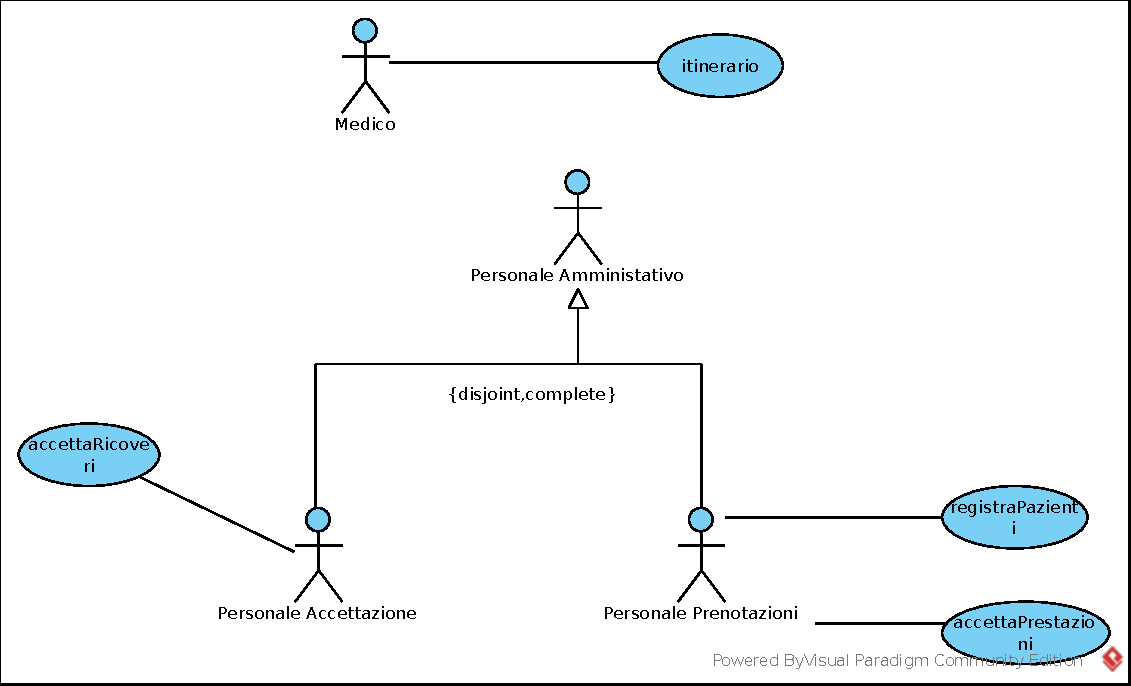
\includegraphics[width=1\textwidth]{./Diagrammi/usecase.pdf}
    \caption{Usecase}
\end{figure}

\newpage

\section{Ristrutturazione}
\subsection{Diagramma delle classi ristrutturato}
\begin{figure}[h]
    \centering
    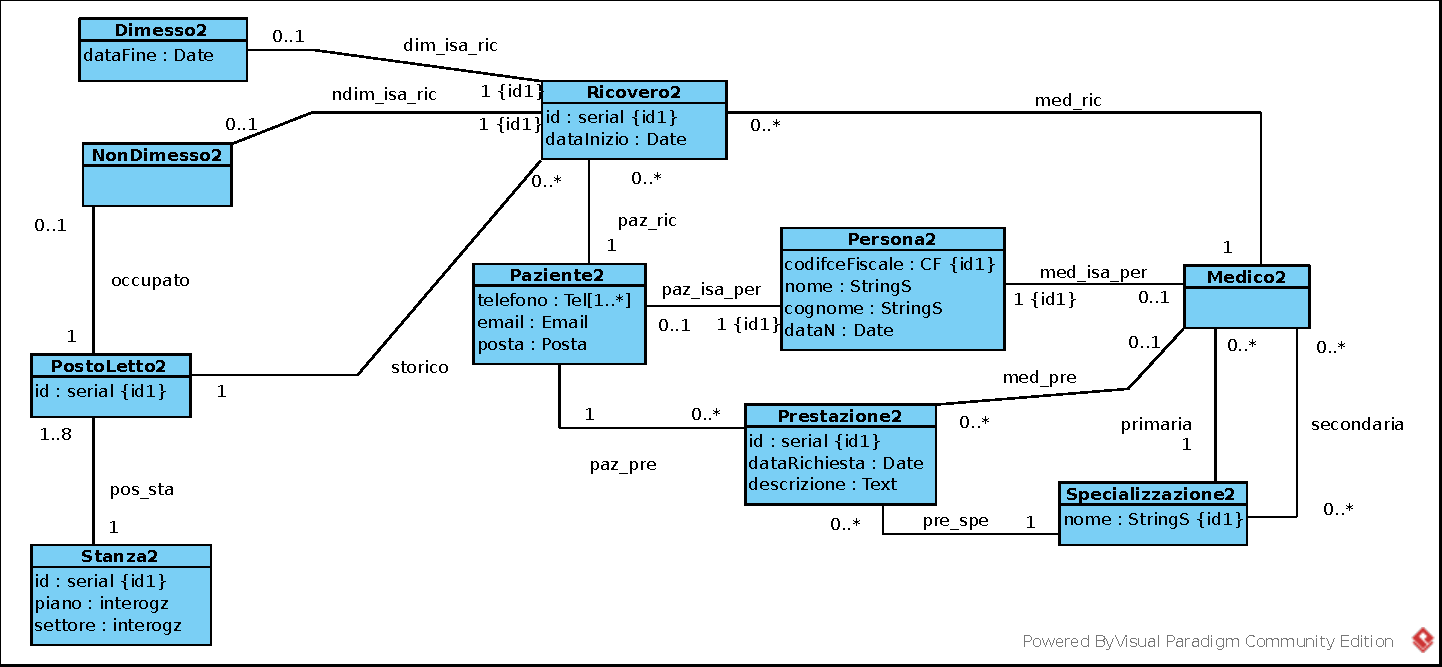
\includegraphics[width=1\textwidth]{./Diagrammi/ristrutturazione.pdf}
    \caption{Ristrutturazione}
\end{figure}

\newpage

\subsection{Dizionario dei dati ristrutturato}

\begin{itemize}
    \item create domain tel as text check $($isTel$($value$))$;
    \item create domain cf as text check $($isCF$($value$))$;
    \item create domain email as text check $($isEmail$($value$))$;
    \item create type posta as $($via IndirizzoNotNull, civico CivicoNotNull$)$;
    \item create domain IndirizzoNotNull as text check $($value is not null$)$;
    \item create domain CivicoNotNull as text check $($value is not null and isCivico$($value$))$
    \item create domain StringS as varchar$($50$)$;
    \item create domain interogz as integer check $($value > 0$)$
\end{itemize}

\newpage

\subsection{Vincoli ristrutturati}

\subsubsection{Vincoli Esterni Aggiunti nella Fase di Ristrutturazione}

\textbf{[V.Occupato\_isa\_Storico]}\\
\[
\forall r,nd,p \; (ndim\_isa\_ric(nd,r) \land occupato(nd,p) \rightarrow storico(r,p))
\]

\textbf{[V.Ricovero\_Dimesso\_Disjoint\_NonDimesso]}\\
\[
\neg \exists r,d,nd \; (ndim\_isa\_ric(nd,r) \rightarrow \neg dim\_isa\_ric(d,r))
\]

\textbf{[V.Ricovero\_Dimesso\_NonDimesso\_Complete]}\\
\[
\forall r \; (\exists nd \; ndim\_isa\_ric(nd,r)) \lor (\exists d \; dim\_isa\_ric(d,r))
\]

\textbf{[V.Persona\_Medico\_Paziente\_Complete]}\\
\[
\forall p \; (\exists m \; med\_isa\_per(m,p)) \lor (\exists paz \; paz\_isa\_per(paz,p))
\]

\subsubsection{Vincoli Esterni Rimasti Invariati dopo la Fase di Ristrutturazione}

\textbf{[V.Prestazione.medico\_giusto]}\\
\[
\forall m,p,s \; (med\_pre(m,p) \land pre\_spe(p,s) \rightarrow (primaria(m,s) \lor secondaria(m,s)))
\]

\textbf{[V.Medico.secondaria\_non\_primaria]}\\
\[
\forall s,m \; (secondaria(m,s) \rightarrow \neg primaria(m,s))
\]

\subsubsection{Vincoli Esterni Modificati durante la Fase di Ristrutturazione}

\textbf{[V.Dimesso.date\_consistente]}\\
\[
\forall r,d \; (dim\_isa\_ric(d,r) \rightarrow \forall d_1,d_2 \; (dataInizio(r,d_1) \land dataFine(d,d_2) \rightarrow d_1 \leq d_2))
\]

\textbf{[V.Ricovero.date\_consistente]}\\
\[
\forall r,dr,paz,per,dp \; (paz\_ric(paz,r) \land paz\_isa\_per(paz,per) \land dataInizio(r,dr) \land dataN(per,dp) \rightarrow dr \geq dp)
\]

\textbf{[V.Prestazione.date\_consistente]}\\
\[
\forall paz,per,pre,d1,d2 \; (paz\_pre(paz,pre) \land paz\_isa\_per(paz,per) \land dataRichiesta(pre,d1) \land dataN(per,d2) \rightarrow d1 \geq d2)
\]

\textbf{[V.Medico.date\_consistente]}\\
\[
\forall m,per,r,d1,d2 \; (med\_ric(m,r) \land dataInizio(r,d1) \land med\_isa\_per(m,per) \land dataN(per,d2) \rightarrow d1 > d2)
\]

\textbf{[V.Paziente.ricovero\_singolo]}\\
\[
\forall p \; (\exists nd,r \; (paz\_ric(p,r) \land ndim\_isa\_ric(nd,r)) \rightarrow \neg \exists nd',r' \; (nd' \neq nd \land r' \neq r \land ndim\_isa\_ric(nd',r') \land paz\_ric(p,r')))
\]

\textbf{[V.Paziente.non\_ricoverato\_da\_se\_stesso]}\\
\[
\forall paz,per,med,r \; (paz\_ric(paz,r) \land med\_isa\_per(med,per) \land paz\_isa\_per(paz,per) \rightarrow \neg med\_ric(med,r))
\]


\newpage

\subsection{Usecases ristrutturati}

\subsubsection{Specifica Use-Case Itinerario}

\textbf{itinerario(): Stanza [0..*]}

\textbf{Pre-condizioni:} nessuna

\textbf{Post-condizioni:}
\begin{itemize}
    \item Non modifica lo spazio estensionale.
    \item Sia \( m \) tale che \texttt{Medico(m)} il medico che si è autenticato nel sistema e che sta usando lo use-case.
    \item Sia \( P = \{p \mid \exists r \; (paz\_ric(p,r) \land med\_ric(m,r) \land NonDimesso(r))\} \).
    \item Sia \( L = \{l \mid \exists n \; (Occupato(n,l) \land n \in P)\} \).
    \item Sia \( S = \{s \mid \exists l \; (pos\_sta(l,s) \land l \in L)\} \).
    \item result = \( S \) (poi in SQL verrà ordinato).
\end{itemize}

\newpage
\subsubsection{Specifica dello Use-Case RegistraPazienti}

\textbf{registrazionePersona(codiceFiscale: CF, nome: Stringa, cognome: Stringa, dataN: Data): Persona}

\textbf{Pre-condizioni:} 
\[
\forall p1 \; (Persona(p1) \rightarrow \neg codiceFiscale(p1,codiceFiscale))
\]

\textbf{Post-condizioni:}
\begin{itemize}
    \item Modifica dello spazio estensionale:
    \item Elementi del dominio di interpretazione: \( \alpha \)
    \item Nuove ennuple:
    \begin{itemize}
        \item \texttt{Persona}(\(\alpha\))
        \item \texttt{codiceFiscale}(\(\alpha\), codiceFiscale)
        \item \texttt{nome}(\(\alpha\), nome)
        \item \texttt{cognome}(\(\alpha\), cognome)
        \item \texttt{dataN}(\(\alpha\), dataN)
    \end{itemize}
    \item result = \texttt{Persona}
\end{itemize}

\textbf{registrazionePaziente(p: Persona, telefoni: Tel [1..*], email: Email, posta: Posta): Paziente}

\textbf{Pre-condizioni:} 
\[
\neg \exists paz \; paz\_isa\_per(paz,p)
\]

\textbf{Post-condizioni:}
\begin{itemize}
    \item Modifica dello spazio estensionale:
    \item Elementi del dominio di interpretazione: \( \alpha \)
    \item Nuove ennuple:
    \begin{itemize}
        \item \texttt{paz\_isa\_per}(\(\alpha\), p)
        \item \texttt{telefono}(\(\alpha\), telefoni)
        \item \texttt{email}(\(\alpha\), email)
        \item \texttt{posta}(\(\alpha\), posta)
    \end{itemize}
    \item result = \texttt{Paziente}
\end{itemize}

\textbf{possibiliMedici(s: Specializzazione): Medico [0..*]}

\textbf{Pre-condizioni:} nessuna

\textbf{Post-condizioni:}
\begin{itemize}
    \item Non modifica lo spazio estensionale.
    \item Sia \( P = \{m \mid primaria(m,s)\} \).
    \item Sia \( S = \{m \mid secondaria(m,s)\} \).
    \item \(|P| > 0 \rightarrow result = P \) \\
    \(|P| = 0 \rightarrow result = S \)
\end{itemize}

\textbf{accettaPrestazione(p: Paziente, s: Specializzazione, dataRichiesta: Data): Prestazione}

\textbf{Pre-condizioni:}
\[
\forall M \; (possibiliMedici\_s(s,M) \rightarrow |M| > 0 \land (\forall d \; (data(adesso,d) \rightarrow dataRichiesta \geq d)))
\]

\textbf{Post-condizioni:}
\begin{itemize}
    \item Modifica dello spazio estensionale:
    \item Elementi del dominio di interpretazione: \( \alpha \)
    \item Nuove ennuple:
    \begin{itemize}
        \item \texttt{Prestazione}(\(\alpha\))
        \item \texttt{dataRichiesta}(\(\alpha\), dataRichiesta)
        \item \texttt{descrizione}(\(\alpha\), descrizione)
        \item \texttt{paz\_pre}(p, \(\alpha\))
        \item \texttt{pre\_spe}(\(\alpha\), s)
    \end{itemize}
    \item result = \( \alpha \)
\end{itemize}

\newpage
\subsubsection{Specifica dello Use-Case AccettaRicoveri}

\textbf{postiLettoLiberi(): PostoLetto[0..*]}

\textbf{Pre-condizioni:} nessuna

\textbf{Post-condizioni:}
\begin{itemize}
    \item Non viene modificato lo spazio estensionale dei dati.
    \item \( L = \{l \mid \neg \exists n \; Occupato(l,n)\} \).
    \item result = \( L \)
\end{itemize}

\textbf{accettaRicoveri(p: Paziente): NonDimesso}

\textbf{Pre-condizioni:} 
\[
(\neg \exists r,nd \; (paz\_ric(p,r) \land NonDimesso(nd) \land ndim\_isa\_ric(nd,r))) \land (\forall L \; (postiLettoLiberi(L) \rightarrow |L| > 0))
\]

\textbf{Post-condizioni:}
\begin{itemize}
    \item Modifica dello spazio estensionale:
    \item Sia \( l \) un elemento a caso in \( \{l \mid \neg \exists n \; Occupato(l,n)\} \).
    \item Elementi del dominio di interpretazione: \( \alpha, \beta \)
    \item Nuove ennuple:
    \begin{itemize}
        \item \texttt{NonDimesso}(\(\beta\))
        \item \texttt{Ricovero}(\(\alpha\))
        \item \texttt{ndim\_isa\_ric}(\(\beta\), \(\alpha\))
        \item \texttt{Storico}(\(\alpha\), l)
        \item \texttt{pos\_sta}(\(\alpha\), l)
    \end{itemize}
    \item result = \( \alpha \)
\end{itemize}

\subsection{Progettazione della base di dati}

\begin{enumerate}
    \item Persona$($\underline{codiceFiscale: cf}, nome: StringS, cognome: StringS, dataN: Data$)$
    \item Paziente(\underline{persona: cf}, telefoni: Tel, email: Email, posta: Posta)
    \begin{enumerate}
        \item foreign key: persona references persona$($codicefiscale$)$
    \end{enumerate}
    \item Medico$($\underline{persona: cf}, specializzazionePrimaria: StringS$)$
    \begin{enumerate}
        \item foreign key: persona references persona$($codicefiscale$)$
        \item foreign key: specializzazionePrimaria references specializzazione$($nome$)$
    \end{enumerate}
    \item SpecializzazioneSecondaria$($\underline{medico: cf, specializzazione: stringaS}$)$
    \begin{enumerate}
        \item foreign key: medico references medico$($persona$)$
        \item foreign key: specializzazione references specializzazione$($nome$)$
    \end{enumerate}
    \item Prestazione$($\underline{id: serial}, dataRichiesta: Date, descrizione: text, paziente: cf, medico*: cf, specializzazioneRichiesta: StringS$)$
    \begin{enumerate}
        \item foreign key: paziente references paziente$($persona$)$
        \item foreign key: medico references medico$($persona$)$
        \item foreign key: specializzazioneRichiesta references specializzazione$($nome$)$
    \end{enumerate}
    \item Ricovero$($\underline{id: serial}, dataInizio: Date, paziente: cf, medico: cf, storico: integer$)$
    \begin{enumerate}
        \item paziente references paziente$($persona$)$
        \item medico references medico$($persona$)$
        \item storico references postoletto$($id$)$
    \end{enumerate}
    \item Dimesso$($\underline{ricovero: integer}, dataFine: Data$)$
    \begin{enumerate}
        \item ricovero references ricovero$($id$)$
    \end{enumerate}
    \item NonDimesso$($\underline{ricovero: integer}$)$
    \begin{enumerate}
        \item ricovero references ricovero$($id$)$
        \item v.\ inclusione: nondimesso$($ricovero$)$ occorre in occupato$($nondimesso$)$
    \end{enumerate}
    \item occupato$($\underline{postoletto: integer}, nonDimesso: integer$)$
    \begin{enumerate}
        \item altra chiave: nonDimesso
        \item foreign key: postoletto references postoletto$($id$)$
        \item foreign key: nonDimesso references nondimesso$($ricovero$)$
    \end{enumerate}
    \item postoletto$($\underline{id: serial}, stanza: integer$)$
    \begin{enumerate}
        \item foreign key: stanza references stanza$($id$)$
    \end{enumerate}
    \item stanza$($\underline{id: serial}, piano: interogz, settore: interogz$)$
    \begin{enumerate}
        \item Domanda: come implemento la molteplicità da 1..8?
    \end{enumerate}
\end{enumerate}


\end{document}
